\documentclass[letterpaper, 12pt, oneside]{book}

%%%%%%%%%%%%%%%%%%%%%%%%%%%%%%%%%%%%%%%%%%%%%%%%%%%%%%%%%%%
%%%%%%%%%%%%%%%%%%%%%%%%% PREAMBULO %%%%%%%%%%%%%%%%%%%%%%%
%%%%%%%%%%%%%%%%%%%%%%%%%%%%%%%%%%%%%%%%%%%%%%%%%%%%%%%%%%%

%%%%%%%%%%%%%%%%%%%%%%%%% PAQUETES %%%%%%%%%%%%%%%%%%%%%%%%

\usepackage{amsmath}                             %Never write a paper without using amsmath for its many new commands 
\usepackage{amssymb}			%
\usepackage{makeidx}			%
\usepackage{graphicx}			%
\usepackage[utf8]{inputenc}			%
\usepackage{hyperref}			%
\usepackage{setspace}			%
\usepackage{cite}			%
%\usepackage{pst-plot}			%
%\usepackage[crop=on]{auto-pst-pdf}
\usepackage{multicol}			%
\usepackage{booktabs}			%
\usepackage{threeparttable}
\usepackage{siunitx}
\usepackage{xfrac}
\usepackage[font=footnotesize,labelfont=bf]{caption} % scriptsize, footnotesize, small, normalsize, large, Large
\usepackage{geometry} % Required for adjusting page dimensions
\usepackage{fancyhdr} % Numeracion y encabezados
\usepackage[intoc, spanish]{nomencl}
%\usepackage[spanish]{babel}			%
%\usepackage[pdf]{pstricks}
%\usepackage{pst-all}
%\usepackage{pst-node}
%\usepackage{pstricks-add}
\usepackage{ipn-cover}					% Formato de portada
\usepackage[x11names]{xcolor}
\usepackage{lineno}

%% Crea los grupos de la nomenclatura. m para las mayusculas, n para las minusculas y g para las letras griegas.
% -----------------------------------------
\usepackage{etoolbox}
\renewcommand\nomgroup[1]{%
  \item[\bfseries
  \ifstrequal{#1}{m}{Mayúsculas}{%
  \ifstrequal{#1}{n}{Minúsculas}{%
  \ifstrequal{#1}{g}{Letras griegas}{}}}%
]}
% -----------------------------------------

\makeindex

\geometry{
	letterpaper, % Hoja tamaño carta
	top=2.5cm, % Top margin
	bottom=2.5cm, % Bottom margin
	left=3.9cm, % Left margin
	right=2.5cm, % Right margin	
	head = 1.0cm,
	foot = 1.0cm,
	includehead, % Include space for a header
	includefoot, % Include space for a footer
	%showframe, % Uncomment to show how the type block is set on the page
}

\pagestyle{fancy} % Enables the custom headers/footers
\fancyhf{}
% Headers
\lhead{AI} % Left header
\chead{AC} % Center header - currently printing the article title
\rhead{AD} % Right header
% Footers
\lfoot{DI} % Left footer
\cfoot{DC} % Center footer
\rfoot{\thepage} % Right footer
\renewcommand{\headrulewidth}{0pt}
\renewcommand{\footrulewidth}{0pt}
\setcounter{secnumdepth}{3} % para que ponga 1.1.1.1 en subsubsecciones
\setcounter{tocdepth}{3} % para que ponga subsubsecciones en el indice

\newskip\smallskipamount \smallskipamount = 3pt plus 1pt minus 1pt
\newskip\medskipamount   \medskipamount  = 6pt plus 2pt minus 2pt
\newskip\bigskipamount   \bigskipamount = 12pt plus 4pt minus 4pt

%\hypersetup{colorlinks,breaklinks,
%    colorlinks,
%    citecolor=[rgb]{0.1,0.	1,0.1},
%    filecolor=[rgb]{0,0.5,0.5},
%    linkcolor=[rgb]{0.2,0.2,0.2},
%    urlcolor=red
%}
\makenomenclature

\singlespacing
%%%%%%%%%%%%%%%%%%%%%
% Definiendo campos %
%%%%%%%%%%%%%%%%%%%%%

\author{M.Sc. Franklin W. Peña-Polo}
\title{Inestabilidades Paramétricas de Ondas en Fluidos.}
\postgraduate{Doctorado en Ciencias en Ingeniería Mecánica}
\degree{F\'ISICO}
\supervisor{Dr. Ignacio Carvajal \\ Dr. Leonardo Sigalotti\\}
\cityandyear{Ciudad de M\'exico, Agosto de 2019}
\logouni{figuras/logo-ipn.png}
\logofac{figuras/logo-esime.png}

\begin{document}

\maketitle


%\singlespacing
%\onehalfspacing
%\doublespacing
\setstretch{1.5} % for custom spacing

\frontmatter
%\thispagestyle{empty}

\begin{center}
%{\large
%.\\
\hfill
\vspace{1.5cm}

{\Large\textbf{Inestabilidades paramétricas de ondas en fluidos en un medio reticulado}}\\
\vspace{2.5cm}
Por\\
Franklin W. Pe\~na Polo\\
\vspace{2.5cm}
Tesis de Grado presentada como requisito parcial para optar\\
al título de Doctor en Ciencias, mención Física\\
\vspace{3.5cm}
INSTITUTO VENEZOLANO DE INVESTIGACIONES CIENTÍFICAS\\
I.V.I.C.\\
CENTRO DE ESTUDIOS AVANZADOS\\
ALTOS DE PIPE\\
\vspace{2.5cm}
JULIO, 2016
%}
\end{center}
\newpage
%\thispagestyle{empty}

La Tesis de Grado de Franklin W. Pe\~na Polo, titulada ``Inestabilidades paramétricas de ondas en fluidos en un medio reticulado'', ha sido aprobada por el jurado, quien no se hace responsable de su contenido, pero la ha encontrado correcta en su calidad y en su forma de presentación en fe de lo cual firman,
\vspace{2cm}
\begin{center}
\begin{multicols}{2}
\noindent\rule{5cm}{0.4pt}\\
Dr.\\
IVIC.

\vspace{2cm}
\noindent\rule{5cm}{0.4pt}\\
Dr.\\
IVIC.

\vspace{2cm}
\noindent\rule{5cm}{0.4pt}\\
Dr.\\
IVIC.

\vspace{2cm}
\noindent\rule{5cm}{0.4pt}\\
Dr.\\
IVIC.

\vspace{2cm}
\noindent\rule{5cm}{0.4pt}\\
Dr.\\
IVIC.

\vspace{2cm}
\noindent\rule{5cm}{0.4pt}\\
Dr.\\
IVIC.

\end{multicols}
\end{center}


\begin{flushright}
Centro de Estudios Avanzado, IVIC.\\
Altos de Pipe, Julio de 2016
\end{flushright}

\newpage
%\thispagestyle{empty}

\begin{center}
Resumen de la Tesis de Grado presentada como requisito parcial par optar
al titulo de Doctor en Ciencias, mención Física\\
\vspace{1.5cm}
\textbf{ONDAS DE FARADAY}\\
\vspace{1.5cm}
Por\\
Franklin W. Peña Polo\\
\vspace{1cm}
Tesis de Grado presentada como requisito parcial para optar\\
al título de Doctor en Ciencias, mención Física\\
\vspace{1cm}
CENTRO DE ESTUDIOS AVANZADOS\\
INSTITUTO VENEZOLANO DE INVESTIGACIONES CIENTÍFICAS\\
I.V.I.C.\\
ALTOS DE PIPE, JULIO, 2016\\
\vspace{1cm}
Leonardo Sigalotti\\
Tutor de Tesis de Grado\\
Abraham Medina\\
Director de la Tesis de Grado\\
\end{center}

Resumen resumen resumen resumen resumen resumen resumen resumen resumen resumen resumen resumen resumen resumen resumen resumen resumen resumen resumen resumen resumen resumen resumen resumen resumen resumen resumen resumen resumen resumen resumen resumen resumen resumen resumen resumen resumen resumen resumen resumen resumen resumen resumen resumen resumen resumen resumen resumen resumen resumen resumen resumen resumen resumen resumen resumen resumen resumen resumen resumen resumen resumen resumen resumen resumen resumen resumen resumen resumen resumen resumen resumen resumen resumen resumen resumen resumen resumen resumen resumen resumen resumen resumen resumen resumen resumen resumen resumen resumen resumen resumen resumen resumen resumen resumen resumen resumen resumen resumen resumen resumen resumen resumen resumen resumen resumen resumen resumen resumen resumen resumen resumen resumen resumen resumen resumen resumen resumen resumen resumen resumen resumen resumen resumen resumen resumen resumen resumen resumen resumen resumen resumen resumen resumen resumen resumen resumen resumen resumen resumen resumen resumen resumen resumen resumen resumen resumen resumen resumen resumen resumen resumen resumen resumen resumen resumen resumen resumen resumen resumen resumen resumen resumen resumen resumen resumen resumen resumen resumen resumen resumen resumen resumen resumen resumen resumen resumen resumen resumen resumen resumen resumen resumen resumen resumen resumen resumen resumen resumen resumen resumen resumen resumen resumen resumen resumen resumen resumen resumen resumen resumen resumen resumen resumen resumen resumen resumen resumen resumen resumen resumen resumen resumen resumen resumen resumen resumen resumen resumen resumen resumen resumen resumen resumen resumen resumen resumen resumen resumen resumen resumen resumen resumen resumen resumen resumen resumen resumen resumen resumen resumen resumen resumen resumen resumen resumen resumen resumen resumen resumen resumen resumen resumen resumen resumen resumen resumen resumen resumen resumen resumen resumen resumen resumen resumen resumen resumen resumen resumen resumen resumen resumen resumen resumen resumen resumen resumen resumen resumen resumen resumen resumen resumen resumen resumen resumen resumen resumen resumen resumen resumen resumen resumen resumen resumen resumen resumen resumen resumen resumen resumen resumen resumen resumen resumen resumen resumen resumen resumen resumen resumen resumen.

%\newpage
%\hfill
\vspace{18cm}
\begin{flushright}
A mi.
\end{flushright}


%\include{5agradecimientos}

\setstretch{1.15} % for custom spacing

\tableofcontents
\listoffigures
\listoftables
\printnomenclature % La 




\newpage

\linenumbers

\mainmatter
\chapter*{Introducción}
\addcontentsline{toc}{chapter}{Introducción}

Al someter un liquido a vibraciones netamente verticales, se observa que en la superficie del liquido se presentan determinados patrones regulares definidos por un cierto rango de frecuencia y amplitudes de la frecuencia de excitación; a este fenómeno se le conoce como \textit{Inestabilidad de Faraday}. El estudio de este tipo de inestabilidad tiene una larga e interesante historia que involucra a dos de los científicos más destacados de la ciencia moderna. A mediados del año 1831, M. Faraday (1791-1867) realizó una serie de experimentos con fluidos sometidos a vibraciones verticales \cite{Faraday1831}. En su bitacora personal Faraday reportó que al hacer vibrar un fluido se presentan una serie de patrones cuadrados en su superficie ``Crispaciones casi siempre cuadrangulares, siempre cuando están bien formadas, pero modificadas por el borde del agua o el líquido, también por el centro de movimiento'' (Faraday, 1831) \cite{Martin1832}. En particular, Faraday señaló que la frecuencia de las ondas presentes en la superficie del liquido era la mitad de la frecuencia de excitación. Casi cuatro décadas después, L. Mathiessen cuestionó la respuesta subarmónica a las vibraciones puramente verticales \cite{Matthiessen1868}, argumentado la existencia de una sincronía entre el forzamiento y las ondas en la superficie del fluido. Esta controversia motivó a Lord Rayleigh (1842-1919) a hacer sus propios análisis, quien mediante un dispositivo bastante ingenioso pudo constatar la afirmación realizada por Faraday \cite{Rayleigh1883b}.\medskip

\begin{figure}
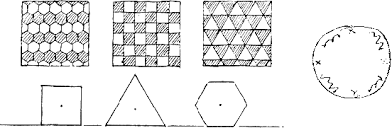
\includegraphics[scale=1]{figuras/faradaysketch.png}
\caption{Izquierda: Bocetos de patrones hexagonales, rectangulares y triangulares realizados por Faraday como posibles interpretaciones de la geometría de las crispaciones. Derecha: Diagrama de la vista superior realizada por Faraday de la distribución de crispaciones en un vaso de agua; ``x'' representa los lugares donde el de agua permanece inmóvil o las crispaciones son débiles, mientras que las líneas onduladas indican una superficie más agitada.\cite{Martin1832}} %sacado de Cavicchi
\end{figure}

En 1954, Benjamin y Ursell desarrollaron una teoría lineal sobre la naturaleza subarmónica de la inestabilidad, realizando la verificación teórica directamente de la hidrodinámica \cite{Benjamin1954}. Sin embargo, el análisis de Benjamin y Ursell se basa en una aproximación de flujo potencial, la cual está restringida únicamente a fluidos sin viscosidad. Si la inestabilidad es generada en un líquido viscoso, una parte de la energía mecánica es disipada debido a esta. Estos efectos generalmente se manejan agregando un amortiguamiento heurístico en la ecuación de Mathieu \cite{Landau1988}, que es proporcional a la viscosidad cinemática $\nu$. La inclusión de dicho término ha sido utilizado ampliamente en varios análisis lineales como los realizados por Müller \cite{Muller1993}; Kumar y Tuckerman \cite{Kumar1994}; Kumar \cite{Kumar1996} y Perlin y Schultz \cite{Perlin2000}. Sin embargo, esta aproximación ignora las capas límite viscosas a lo largo de las paredes del contenedor y debajo de la superficie, donde se produce una disipación adicional. \medskip

La descripción matemática completa del problema involucra las ecuaciones de Navier-Stokes en un dominio con una superficie libre, donde las amplitudes de los modos normales se desacoplan y cumplen en primera aproximación de la ecuación de Mathieu, la cual es una ecuación diferencial ordinaria de segundo orden no autónoma. En matemáticas, un sistema no autónomo es un sistema de ecuaciones diferenciales ordinarias que depende explícitamente de la variable independiente. En este caso, la falta de autonomía está dada por el forzamiento externo que influye en los parámetros del fluido cuando se inicia el comportamiento oscilante. Benjamin y Ursell pudieron utilizar las propiedades de estabilidad conocidas de la ecuación de Mathieu para confirmar el punto de vista de Faraday y Rayleigh. Al tipo de inestabilidad presente en la ecuación de Mathieu se le llama \textit{Inestabilidad paramétrica}, y es conocida por estar presente en diversos sistemas como osciladores electrónicos, ondas de Langmuir en plasma y hasta en el comportamiento estocástico de un conjunto de precios sectoriales internacionales. El experimento mas representativo de este fenómeno es el péndulo excitado paramétricamente. Si el pivote del péndulo oscila verticalmente, el péndulo comenzará a oscilar horizontalmente con la mitad de la frecuencia de excitación para algunas amplitudes y frecuencias. En este ejemplo, así como en el experimento de Faraday, la aceleración gravitacional efectiva es el parámetro externo impulsador. La ecuación de Mathieu lleva el nombre del matemático francés E. L. Mathieu (1825-1890), quien en su trabajo original de 1868 muestra como resolver la ecuación de onda bidimensional para el movimiento de una membrana elíptica \cite{Mathieu1868}.\medskip

Es interesante notar que Lord Rayleigh reconoció el experimento de Faraday como una inestabilidad paramétrica \cite{Rayleigh1883a}. En su trabajo de 1883, en realidad analizó la ecuación de Mathieu en presencia de amortiguamiento y encontró una condición necesaria para la respuesta subarmónica. Más tarde \cite{Rayleigh1887} elaboró sobre el tema inspirado en el trabajo del físico estadounidense G. W. Hill (1838-1914) \cite{Hill1886} sobre una generalización de la ecuación de Mathieu relativa al movimiento de la luna bajo la influencia del sol y la tierra.\medskip

En las ultimos 50 años se ha realizado un esfuerzo por ampliar el análisis de Benjamin y Ursell a amplitudes finitas mediante la incorporación de no linealidades débiles. Por su parte, Dodge \textit{et al} encontraron congruencia entre sus medidas del umbral de amplitudes \cite{Dodge1965} y las predicciones no viscosas de Benjamin y Ursell, a excepción de tres discrepancias: (i) la teoría para liquidos no viscosos predice cero en el ubral de amplitud en resonancia, mientras que las ondas reales deben superar un umbral viscoso; (ii) el ancho de banda medido es más estrecho que la predicción no viscosa; y (iii) la frecuencia de resonancia medida es menor que la predicción no viscosa. Estas discrepancias ponen en evidencia los efectos viscosos. Dodge \textit{et al} también informaron mediciones de amplitud de ondas en cilindros circulares aproximadamente dos veces más grandes que las nuestras. Virnig \textit{et al} midieron las amplitudes de ondas en estado estacionario en grandes cilindros rectangulares en los que los efectos viscosos y capilares eran pequeños \cite{Virnig1988} obteniendo resultados que coinciden razonablemente con los cálculos de Gu \textit{et al} \cite{Gu1988}. Con el creciente interés en la dinámica no lineal y el caos temporal, el experimento de Faraday ha ganado un interés más amplio. Keolian \textit{et al} \cite{Keolian1981} observó un estado caótico en una célula anular fuertemente impulsada. Dos años después de que Gollub y Meyer \cite{Gollub1983} estudiaran la transición al caos de un modo único en una celda circular. Ciliberto y Gollub \cite{Ciliberto1984, Ciliberto1985} mostraron cómo la competencia entre dos modos superpuestos puede conducir al caos. Además, Simonelli y Gollub \cite{Simonelli1989} estudiaron las interacciones de dos modos casi degenerados por simetría.

Mas recientemente, la inestabilidad de Faraday se ha estudiado ampliamente, tanto teóricamente \cite{Benjamin1954}, \cite{Miles1984}, \cite{Holmes1984}, \cite{Meron1986}, \cite{Gu1987}, \cite{Armbruster1989} \cite{Feng1989} \cite{Umeki1989} \cite{Miles1990}, \cite{Miles1993}, \cite{Bechhoefer1996}, \cite{Muller1997}, \cite{Muller1998a}, \cite{Mancebo2002}, \cite{Huepe2006}, \cite{Perinet2010}, \cite{Perinet2012}, y experimentalmente \cite{Douady1990}, \cite{Edwards1994}, \cite{Bechhoefer1995}, \cite{Kityk2002}, \cite{Westra2003}, \cite{Residori2007}, \cite{NguyemThuLam2011} para el estudio de la formación de patrones. A partir de una elección adecuada de los parámetros experimentales, se pueden observar varios patrones distintos, que consisten en un conjunto de figuras geométricas ordenadas como rayas, cuadrados, triángulos y hexágonos. Patrones de superredes Kudrolli et al. \cite{Kudrolli1998} y estructuras localizadas Arbell y Fineberg \cite{Arbell2000}, \cite{Arbell2002} también se han observado utilizando forzamientos de dos frecuencias. Comprender los tipos de patrones que se forman es un desafío. El umbral de inestabilidad y los patrones observados dependen de la viscosidad y la tensión superficial del fluido, la aceleración forzada $\Gamma$ y la forma y tamaño del recipiente. Además, las fluctuaciones en la frecuencia y amplitud de la fuerza impulsora pueden llevar un patrón existente a un estado mixto con una fracción de caos espacio-temporal (Kudrolli y Gollub 1996).

%---------------------------------

La investigación mencionada anteriormente aborda el límite de las relaciones de aspecto bajas, es decir, cuando la longitud de onda es comparable al tamaño del sistema. En este caso, solo unos pocos modos se excitan simultáneamente y la dinámica es de baja dimensión. Gran parte del interés actual en el experimento de Faraday se debe a sus posibilidades como sistema con muchos grados de libertad. Para este propósito, el experimento de Faraday tiene dos ventajas principales; la relación de aspecto puede variarse simplemente variando la frecuencia, y la dinámica puede investigarse visualmente.

Un resultado sorprendente para las relaciones de aspecto altas es la observación de que el relieve de la superficie puede tomar la forma de patrones ordenados que se asemejan mucho a los cristales bidimensionales. Sin embargo, la verdadera sorpresa es que estos patrones no se limitan a las celdas de una geometría particular. Para relaciones de aspecto altas, los límites se vuelven menos importantes y la geometría es la del plano infinito. Esto ya lo notó Faraday. Al estudiar el patrón cuadrado observa: `Evidentemente, no es causado por ondas interferentes, aunque puede resolverse en ellas. ... Además, por irregulares que sean los bordes, la disposición puede hacerse cuadrangular '[19, §58]. Ezerskii et al. (1986) informaron recientemente un patrón cuadrado (1986) en una geometría circular. [14, 15]. En el mismo año, Aleksandrov et al. [1] encontró un patrón hexagonal para las amplitudes de la unidad debajo de aquellas para las cuales observaron el patrón cuadrado. La selección de patrones para las relaciones de aspecto intermedias ha sido investigada por Douady y Fauve [10, 11]. Notamos que se pueden introducir múltiples números de onda críticos a través de un forzado con más de un componente de frecuencia. Esto favorece el sistema Faraday de otros sistemas de formación de patrones como la convección de Rayleigh-Benard y permite la ingeniería de patrones [13].

Varios autores han estudiado experimentalmente el desglose del patrón cuadrado a un estado desordenado a medida que aumenta la amplitud de la unidad. Tuffilaro y col. [65] estudió el longitud de correlación en función de la amplitud de la unidad y encontró un punto de transición bien definido. Por encima de la transición se encuentra el caos espacio-temporal o la turbulencia débil, es decir, se pierde la coherencia espacial pero la dinámica sigue dominada por una escala de longitud única. Ezerskii y col. [15, 16, 17] encontraron que la transición está mediada por el inicio de modulaciones transversales de longitud de onda larga. Las propiedades de transporte de las turbulentas olas de Faraday se han estudiado recientemente [59, 48]. Estos aspectos se revisan en las Refs. [22, 24] y [25].

Varios trabajadores han realizado intentos teóricos para comprender la formación del patrón y la transición al caos espacio-temporal. El más ambicioso parece ser el de Milner [51], que aplica el método de escalas múltiples para derivar las ecuaciones de amplitud. Sobre la base de las consideraciones energéticas, concluye que el estado preferido es el patrón cuadrado. Esto está en contradicción con la observación antes mencionada de un patrón hexagonal [1], y con los resultados experimentales reportados en la presente tesis. La teoría de Levin et al. [42] predice patrones hexagonales y cuadrados, pero sus métodos y presunciones parecen muy burdos. Ezerskii, Rabinovich y col. [15, 16, 54, 55] aplican principalmente su versión de las ecuaciones de amplitud al problema del caos e intermitencia espacio-temporal.

En esta tesis presentamos un estudio experimental del sistema de Faraday de alta relación de aspecto. Se hace hincapié en la observación de una serie de patrones cristalinos de diferente simetría. En particular, el descubrimiento de un estado cuasicristalino es de interés, ya que, según nuestro conocimiento, es el primer patrón de este tipo que se encuentra en un sistema hidrodinámico. El resto de la parte I de la tesis se organiza de la siguiente manera. En sec. 2 se desarrollan la hidrodinámica y la teoría lineal. La sección 3 ofrece una breve reseña histórica de los cuasicristales. En sec. 4 describimos la configuración experimental, y en la Sec. 5 se analiza el sistema óptico. En sec. 6 informamos nuestros resultados sobre la relación de dispersión, las tasas de amortiguamiento y la amplitud crítica, mientras que la Sec. 7 está dedicado a los patrones cristalinos y al diagrama de fases. La sección 8 contiene una discusión de la teoría no lineal. Cerramos esta parte de la tesis en la Sec. 9 con la conclusión.

\chapter{Marco Teórico}
%%%%%%%%%%%%%%%%%%%%%%%%%%%%%%%%%%%%%%%%%%%%%%%%%%%%%%%%%%%%%%%%%%%%%%%%%%%%%%%%%%%%%%%%%%%%%%
%%%%%%%%%%%%%%%%%%%%%%%%%%%%%%%%%%%%%%%%%% SECCION %%%%%%%%%%%%%%%%%%%%%%%%%%%%%%%%%%%%%%%%%%%
%%%%%%%%%%%%%%%%%%%%%%%%%%%%%%%%%%%%%%%%%%%%%%%%%%%%%%%%%%%%%%%%%%%%%%%%%%%%%%%%%%%%%%%%%%%%%%

%\begin{minipage}{\textwidth}
%{\normalsize
%%\tiny \scriptsize \footnotesize \small \normalsize \large \Large \LARGE \huge \Huge
%
%1. Introducción\\
%2. Marco Teórico\\
%2.1 Ondas de superficie y ondas de Faraday\\
%2.2 Análisis Lineal\\
%2.3 Análisis No-lineal\\
%2.4. Simulaciones numéricas\\
%3. Montaje Experimental\\
%3.1 Diseño experimental\\
%3.2 Patrones de Faraday en Reticulados\\
%3.3 Patrones de Faraday en Contenedores\\
%3.4 Gotas Suspendidas y Coalescencia de Gotas suspendidas\\
%4. Resultados: Patrones de Faraday en Reticulados\\
%4.1 Patrones de Faraday en reticulados de celdas cuadradas\\
%4.2 Patrones de Faraday en reticulados de celdas triangulares\\
%4.3 Patrones de Faraday en reticulados de celdas hexagonales\\
%4.4 Efectos de las dimensiones de las celdas\\
%4.5 Efectos del tipo de material\\
%4.6 Efectos de la densidad y viscosidad del líquido\\
%4.7 Implicaciones teóricas\\
%5. Resultados: Patrones de Faraday en Contenedores para Capas Multifásicas\\
%5.1 Deformación de la interface para fases aceite-agua\\
%5.2 Comparación con simulaciones numéricas\\
%6. Gotas Suspendidas\\
%7. Implicaciones Topológicas\\
%8. Discusión de los Resultados\\
%9. Conclusiones\\
%}
%\end{minipage}

\section{Descripción de un fluido}

En esta sección plantearemos las ecuaciones fundamentales de la hidrodinámica, necesarias para la descripción del experimento de Faraday \cite{Faraday1831}. En mecánica de fluidos, las ecuaciones que rigen el comportamiento de un fluido \cite{Landau1987, Batchelor2002, Lamb1975}, en su forma más general son:

\begin{equation} \label{eq201}
   \frac{\partial \rho}{\partial t} + \nabla \cdot (\rho \vec{v}) = 0,
\end{equation}

\nomenclature[g]{$\rho$}{Densidad}
\nomenclature[n]{$t$}{Tiempo}
\nomenclature[g]{$\nabla$}{Operador diferencial vectorial}
\nomenclature[n]{$\vec{v}$}{Vector velocidad}

\begin{equation}\label{eq202}
   \rho \left[\frac{\partial \vec{v}}{\partial t} + (\vec{v} \cdot \nabla ) \vec{v}\right] = \vec{F} - \nabla p + \mu  \nabla^2 \vec{v} + (\zeta + \frac{1}{3} \mu) \nabla (\nabla \cdot \vec{v}).
\end{equation} \medskip

\nomenclature[m]{$\vec{F}$}{Fuerza}
\nomenclature[n]{$p$}{Presión}
\nomenclature[g]{$\mu$}{Viscosidad dinámica}
\nomenclature[g]{$\zeta$}{Segunda viscosidad}

\noindent La ecuación \ref{eq201} expresa el principio de la conservación de la materia y se conoce como la ecuación de continuidad \index{ecuación de continuidad}, donde $\rho$ es la densidad del fluido y $\vec{v} = v_x\hat{i} + v_y\hat{j} + v_z\hat{k}$ la velocidad del flujo. la ecuación \ref{eq202} combina los principios de conservación de la mecánica y la termodinámica aplicados a un volumen de fluido llamada ecuación de Navier-Stokes \index{ecuación de Navier-Stokes}, donde $\vec{F}$ y $p$ es una fuerza y la presión que actúa sobre el volumen de fluido, respectivamente, $\mu$ es la viscosidad dinámica y $\zeta$ es la segunda viscosidad.

En la mayoría de los casos de interés, un líquido convencional, tal como el agua, es incompresible. Un fluido, se dice que es incompresible, cuando la densidad de masa $\rho$ de un elemento de volumen $V$ no cambia notablemente con el tiempo, y ademas, tiene la capacidad de oponerse a la comprensión, es decir, el volumen del fluido permanece constante ante las variaciones de la presión, así

\begin{equation}\label{eq203}
   \frac{d \rho}{d t} = 0.
\end{equation}

Generalmente la distribución de densidad inicial de un fluido incompresible es espacialmente uniforme. Por lo tanto, podemos decir que la distribución de densidad es constante en el tiempo y uniforme en el espacio.

Debido a que el término relacionado con la segunda viscosidad resulta de mayor importancia en casos tales como fluidos compresibles, ondas de choque, propagación de sonido en un fluido Newtoniano como el de la ley de Stokes de la atenuación del sonido \cite{Anderson, Dukhin, Litovitz}, podemos omitir este.

Suponiendo que la fuerza $\vec{F}$ que actúa sobre el volumen de fluido, presente en la ecuación \ref{eq202}, es de naturaleza conservativa, es decir,

\begin{equation}\label{eq204}
   \vec{F} = -\rho \nabla \it\Psi,
\end{equation}

\nomenclature[n]{$\psi$}{Potencial de energía}

\noindent donde $\it\Psi$ es la energía potencial por unidad de masa y $\rho \it\Psi$ es la energía potencia por unidad de volumen. Ademas, si asumimos que en seno del fluido no existen fuertes variaciones de temperatura, podemos suponer que la viscosidad es espacialmente uniforme, de tal manera que la ecuación de Navier-Stokes para un fluido incompresible se reduce a

\begin{equation}\label{eq205}
   \rho \left[\frac{\partial \vec{v}}{\partial t} + (\vec{v} \cdot \nabla ) \vec{v}\right] = - \nabla p  - \rho \nabla \it\Psi + \rho \nu \nabla^2 \vec{v},
\end{equation}

\noindent donde $\nu=\tfrac{\mu}{\rho}$ es la viscosidad cinemática. En términos generales, el momentum se difunde una distancia del orden $\sqrt{\nu t}$ metros en $t$ segundos como consecuencia de la viscosidad. La viscosidad cinemática del agua a 20$^o$C es de aproximadamente $1.0 \times 10^{-6}$ m$^2$/s \cite{Batchelor2002}. De ello se deduce que la difusión del momento viscoso en agua es un proceso relativamente lento.

El conjunto completo de ecuaciones que gobiernan a un fluido incompresible entonces son:

\begin{equation}\label{eq206}
   \nabla \cdot \vec{v} = 0,
\end{equation}

\begin{equation}\label{eq207}
   \frac{\partial \vec{v}}{\partial t} + (\vec{v} \cdot \nabla ) \vec{v} = - \frac{\nabla p}{\rho}  - \nabla \it\Psi + \nu \nabla^2 \vec{v}.
\end{equation}

Aquí, $\rho$ y $\nu$ son consideradas constantes conocidas, y $\it\Psi(\vec{r},t)$ la asumiremos como una función conocida. Por lo tanto, tenemos cuatro ecuaciones: la ecuación \ref{eq206}, además de las tres componentes de la ecuación \ref{eq207}, para cuatro incógnitas, que serian, la presión, $p(\vec{r},t)$ y las tres componentes de la velocidad, $\vec{v}(\vec{r},t)$. Debemos tener en cuenta que una ecuación de conservación de energía es redundante en el caso de flujo de fluido incompresible.

%%%%%%%%%%%%%%%%%%%%%%%%%%%%%%%%%%%%%%%%%%%%%%%%%%%%%%%%%%%%%%%%%%%%%%%%%%%%%%%%%%%%%%%%%%%%%%
%%%%%%%%%%%%%%%%%%%%%%%%%%%%%%%%%%%%%%%%% SUBSECCION %%%%%%%%%%%%%%%%%%%%%%%%%%%%%%%%%%%%%%%%%
%%%%%%%%%%%%%%%%%%%%%%%%%%%%%%%%%%%%%%%%%%%%%%%%%%%%%%%%%%%%%%%%%%%%%%%%%%%%%%%%%%%%%%%%%%%%%%

\subsection{Ondas de superficie}      

Consideremos un volumen de agua contenido por un recipiente, el cual posee una profundidad $d$, sobre la superficie del planeta tierra. Asumiendo que este cuerpo es lo suficientemente pequeño en comparación con la Tierra, tal que su superficie imperturbable es aproximadamente plana. Con la coordenada cartesiana $z$ orientada en la vertical, con $z = 0$ correspondiente a la superficie antes mencionada. Supongamos que una onda de pequeña amplitud se propaga horizontalmente a través del agua, siendo $v(r, t)$ el campo de velocidades asociado.

%\begin{figure}[ht]
%\centerline{
%\begin{minipage}{0.8\textwidth}
%\centering
%\psset{xunit=2pt, yunit=2pt}
%\begin{pspicture*}(-55,-10)(55,20)
%   \psplot[linecolor=blue!80, linewidth=1pt, fillcolor=blue!80,fillstyle=solid]{-32}{32}{ x 0.02 div cos}
%%   \psplot[linecolor=blue!80, linewidth=1pt, fillcolor=blue!80,fillstyle=solid]{31.416}{34.478}{ x 0.02 div cos}
%   %\psplot[linecolor=blue, linewidth=1pt, fillcolor=red,fillstyle=solid]{-34.478}{34.478}{ x 0.02 div cos}
%   \psframe[linecolor=blue!80,fillcolor=blue!80, fillstyle=solid](-33,-7)(33,-.6)
%   \psline[linewidth=1pt,linecolor=black!60](33,-7)(33,3)
%   \psline[linewidth=1pt,linecolor=black!60](-33,-7)(-33,3)
%   \psline[linewidth=1pt,linecolor=black!60](-33,-7)(33,-7)
%   \uput[-135](-35,1.5){\footnotesize $d$}
%   \psline[linewidth=.5pt,linecolor=black]{->}(-38,0)(-38,3)
%   \psline[linewidth=.5pt,linecolor=black]{->}(-38,-4)(-38,-7)
%   \psline[linewidth=.5pt,linecolor=black](-33,-7)(-39,-7)
%   \psline[linewidth=.5pt,linecolor=black](-33,3)(-39,3)
%   \psset{trigLabels=true,labelFontSize=\scriptstyle}
%   \uput[-135](-49.5,10){\footnotesize{ $^x$}}
%   \psline[linewidth=.5pt,linecolor=black]{->}(-48,10)(-51,7)
%   \uput[-135](-40,11){\footnotesize $^y$}
%   \psline[linewidth=.5pt,linecolor=black]{->}(-48,10)(-42,10)
%   \uput[-135](-46.5,18){\footnotesize $^z$}
%   \psline[linewidth=.5pt,linecolor=black]{->}(-48,10)(-48,15)
%%   \uput[-135](52,4){\footnotesize{$z=0$}}
%%   \psline[linewidth=.5pt,linecolor=black!70,linestyle=dashed]{->}(30,0)(38,0)
%%   \uput[-135](52,-3){\footnotesize{$z=h$}}
%%   \psline[linewidth=.5pt,linecolor=black!70,linestyle=dashed]{->}(30,-7)(38,-7)
%   %\psarc[fillcolor=white]{->}(0,0){2}{-90}{90}
%   %\pscircle(0,0){1}
%   %\pswedge[fillstyle=solid,fillcolor=red](0,0){0.5}{0}{45}
%   %\psellipse(0,0)(10,5)
%\end{pspicture*}
%\caption{Ondas de gravedad en la superficie de un volumen de líquido contenido en un recipiente de profundidad $d$.} 
%\end{minipage}
%}
%\end{figure}

Debido a que el agua es un liquido en esencia incompresible, las ecuaciones de movimiento están descritas por \ref{eq206} y \ref{eq207}, las cuales podemos reescribir como:

\begin{equation}\label{eq208}
   \nabla \cdot \vec{v} = 0,
\end{equation}

\begin{equation}\label{eq209}
   \rho \frac{\partial \vec{v}}{\partial t} + \rho (\vec{v} \cdot \nabla ) \vec{v} = - \nabla p - \rho g  \hat{e}_{z} + \mu  \nabla^2 \vec{v},
\end{equation}

\noindent donde $g$ es la aceleración debida a la gravedad terrestre y se ha reemplazado $\nabla \it\Psi = g \hat{e}_{z}$ el potencial gravitatorio. La presión la podemos escribir

\begin{equation}\label{eq210}
   p(\vec{r}, t) = p_0 - \rho gz + p_1(\vec{r}, t),
\end{equation}

\noindent siendo $p_0$ es la presión atmosférica y $p_1$ la presión de perturbación debida a la onda. En ausencia de la onda, la presión del agua a una profundidad $h$ por debajo de la superficie es $p_0+\rho g h$. Sustituyendo en \ref{eq209} y despreciando los términos de segundo orden, tenemos

\begin{equation}\label{eq211}
   \rho \frac{\partial \vec{v}}{\partial t} \simeq - \nabla p_1 + \mu  \nabla^2 \vec{v},
\end{equation}

Por otra parte, despreciando la viscosidad, lo cual no es seria un error si consideramos que, por ejemplo, para el agua la viscosidad es despreciable siempre que $\lambda \gg (\tfrac{v^2}{g})^{\tfrac{1}{3}} \sim 5 \times 10^{-5}$m. Así la ecuación \ref{eq211} se reduce a

\begin{equation}\label{eq212}
   \rho \frac{\partial \vec{v}}{\partial t} \simeq - \nabla p_1.
\end{equation}

Si tomamos el rotor de esta ecuación obtenemos que 

\begin{equation}\label{eq213}
   \rho \frac{\partial \vec{\omega}}{\partial t} \simeq 0,
\end{equation}

\noindent siendo $\vec{\omega} = \nabla \times \vec{v}$ la vorticidad. Lo que nos dice que el campo de velocidad asociado con la onda es irrotacional. La ecuación \ref{eq213} puede ser satisfecha haciendo 

\begin{equation}\label{eq214}
   \vec{v} = \nabla \phi,
\end{equation}

\noindent donde $\phi(\vec{r},t)$ es el potencial de velocidad. Sin embargo, aplicando esto a la ecuación \ref{eq208}, se obtiene que el potencial de velocidad satisface la ecuación de Laplace,

\begin{equation}\label{eq215}
   \nabla^2 \phi = 0.
\end{equation}

\noindent Finalmente, de las ecuaciones \ref{eq212} y \ref{eq214} se obtiene que la presión en superficie perturbada es

\begin{equation}\label{eq216}
   p_1 = - \rho \frac{\partial \phi}{\partial t}.
\end{equation}

%%%%%%%%%%%%%%%%%%%%%%%%%%%%%%%%%%%%%%%%%%%%%%%%%%%%%%%%%%%%%%%%%%%%%%%%%%%%%%%%%%%%%%%%%%%%%%
%%%%%%%%%%%%%%%%%%%%%%%%%%%%%%%%%%%%%%% SUBSUBSECCION %%%%%%%%%%%%%%%%%%%%%%%%%%%%%%%%%%%%%%%%
%%%%%%%%%%%%%%%%%%%%%%%%%%%%%%%%%%%%%%%%%%%%%%%%%%%%%%%%%%%%%%%%%%%%%%%%%%%%%%%%%%%%%%%%%%%%%%

\subsubsection{Condiciones de borde}

Ahora debemos considerar las condiciones físicas a ser satisfechas en los limites superior e inferior del agua. El agua está delimitada por la parte de abajo por una superficie sólida situada en $z = -d$. Dado que el agua debe permanecer siempre en contacto con esta superficie, la restricción física adecuada en el límite inferior es $v_z|_{z=-h}= 0$, es decir, la velocidad normal es cero en el límite inferior, o lo que es lo mismo

\begin{equation} \label{eq217}
   v_z|_{z=-h} = \left. \frac{\partial \phi}{\partial z} \right|_{z=-d} = 0.
\end{equation}

El límite superior del agua es un poco más complicado, debido a que es una superficie libre. Considerando $\zeta$ como el desplazamiento vertical de esta superficie debido a la onda, tenemos que 

\begin{equation} \label{eq218}
   v_z|_{z=0} = \left. \frac{\partial \phi}{\partial z} \right|_{z=0} = \frac{\partial \zeta}{\partial t}.
\end{equation}

La restricción física adecuada para el límite superior es que la presión del agua debe ser igual a la presión atmosférica, ya que no puede haber una discontinuidad de presión a través de una superficie libre, esto en ausencia de la tensión superficial. En consecuencia, a partir de la ecuación \ref{eq210}, obtenemos

\begin{equation}\label{eq219}
   p_1|_{z=0} = \rho g\zeta,
\end{equation}

\noindent lo cual implica que

\begin{equation}\label{eq220}
   \left. \frac{\partial p_1}{\partial t} \right|_{z=0} = \rho g \frac{\partial \zeta}{\partial t} = - \left. \rho g \frac{\partial \phi}{\partial z} \right|_{z=0}, 
\end{equation}

\noindent donde también se ha empleado la ecuación \ref{eq218}. Combinando esta expresión con la ecuación \ref{eq216} obtenemos,

\begin{equation}\label{eq221}
   \left. \frac{\partial \phi}{\partial z} \right|_{z=0} = - g^{-1} \left. \frac{\partial^2 \phi}{\partial^2 t} \right|_{z=0},
\end{equation}

\noindent la cual es la condición para la superficie libre \cite{Lamb1975}.

Suponiendo una solución a la ecuación de onda \ref{eq215} de la forma

\begin{equation}\label{eq222}
  \phi(\vec{r}, t) = F(z) \cos(\omega t - k x).
\end{equation}

\noindent esta solución corresponde en realidad a la propagación de onda plana de vector de onda $\vec{k} = k \hat{e}_x$, frecuencia angular $\omega$ y amplitud $F(z)$. Sustituyendo en la ecuación \ref{eq215}, obtenemos, 

\begin{equation}\label{eq223}
  \frac{d^2 F}{d z^2} - k^2 F = 0,
\end{equation}

\noindent cuyas soluciones independientes son $e^{(+k z)}$ y $e^{(-k z)}$. Por lo tanto, una solución general de \ref{eq215} toma la forma

\begin{equation}\label{eq224}
   \phi(x, z, t) = A e^{k z}\cos(\omega t - k x) + B e^{-k z}\cos(\omega t - k x),
\end{equation}

\noindent donde $A$ y $B$ son constantes arbitrarias. La condición de frontera \ref{eq217} satisface la condición de que $B = A e^{(-2kd)}$, dando

\begin{equation}\label{eq225}
   \phi(x, z, t) = A \left[e^{k z}+e^{-k(z+2d)}\right] \cos(\omega t - k x),
\end{equation}

\noindent la condición de frontera \ref{eq221} produce entonces

\begin{equation}\label{eq226}
   A k \left(1-e^{-2kz}\right)\cos(\omega t - k x) = A \frac{\omega^2}{g} \left(1+e^{-2kz}\right)\cos(\omega t - k x),
\end{equation}

\noindent la cual se reduce a la relación de dispersión 

\begin{equation}\label{eq227}
   \omega^2 = g k \tanh(k d).
\end{equation}

%%%%%%%%%%%%%%%%%%%%%%%%%%%%%%%%%%%%%%%%%%%%%%%%%%%%%%%%%%%%%%%%%%%%%%%%%%%%%%%%%%%%%%%%%%%%%%
%%%%%%%%%%%%%%%%%%%%%%%%%%%%%%%%%%%%%%% SUBSUBSECCION %%%%%%%%%%%%%%%%%%%%%%%%%%%%%%%%%%%%%%%%
%%%%%%%%%%%%%%%%%%%%%%%%%%%%%%%%%%%%%%%%%%%%%%%%%%%%%%%%%%%%%%%%%%%%%%%%%%%%%%%%%%%%%%%%%%%%%%

\subsubsection{Energía de las ondas de gravedad}

La velocidad de fase es la velocidad aparente de una fase determinada de una onda. La velocidad de fase está dada en términos de la frecuencia angular de la onda $\omega$ 
y del vector de onda $k$, por la relación \cite{Narayanan2015},

\begin{equation}\label{eq228}
   v_p = \frac{\omega}{k},
\end{equation}

\noindent Empleando la ecuación \ref{eq227} podemos escribir la velocidad de fase de una onda de gravedad que se propagando horizontalmente a través de un volumen de agua 
de profundidad $d$ como,

\begin{equation}\label{eq229}
   v_p = (gd)^{1/2} \left[\frac{\tanh(kd)}{kd}\right]^{1/2}.
\end{equation}

La tasa a la cual viaja la energía almacenada en la onda es la velocidad de grupo, la cual podemos escribir como \cite{Narayanan2015},

\begin{equation}\label{eq230}
   v_g = \frac{\partial \omega}{\partial k}
\end{equation}

\noindent así, empleando la ecuacion \ref{eq227} se tiene que, 

\begin{equation}\label{eq231}
   v_g = \frac{1}{2}\frac{(g\tanh(kd)+gkd(1-\tanh^2(kd)))}{\sqrt{(gk\tanh(kd))}},
\end{equation}

\noindent además, la razón entre la velocidad de grupo y la velocidad de fase es

\begin{equation}\label{eq232}
   \frac{v_p}{v_g} = \frac{1}{2} \left[1 + \frac{2kd}{\sinh(2kd)}\right].
\end{equation}

Se debe tener en cuenta que ni la velocidad de fase ni la velocidad de grupo de una onda de gravedad pueden exceder un cierto valor critico $(gd)^{\frac{1}{2}}$. Por otra parte, el campo de desplazamiento y el campo de velocidad asociados a una onda de gravedad plana de número de onda $k\hat{e}_x$, frecuencia angular $\omega$, y amplitud $a$, son

\begin{eqnarray}
   \xi_x(x,z,t)& = & -a \frac{\cosh[k(z+d)]}{\sinh(kd)}\cos(\omega t - kx),\label{eq233}\\
   \xi_x(x,z,t)& = & -a \frac{\cosh[k(z+d)]}{\sinh(kd)}\cos(\omega t - kx),\label{eq234}\\
   v_x(x,z,t) & = & a \omega \frac{\cosh[k(z+d)]}{\sinh(kd)}\sin(\omega t - kx),\label{eq235}\\
   v_z(x,z,t) & = & a \omega \frac{\sinh[k(z+d)]}{\sinh(kd)}\cos(\omega t - kx),\label{eq236}
\end{eqnarray}

\noindent La energía cinética media por unidad de superficie asociada con una onda de gravedad se define como

\begin{equation}\label{eq237}
      K = \left\langle \int_{- d}^\zeta \frac{1}{2} \rho v^{2}dz \right\rangle,
\end{equation} 

\noindent dónde

\begin{equation}\label{eq238}
   \zeta(x, t) = a \sin(\omega t -kx)
\end{equation}

\noindent que es el desplazamiento vertical de la superficie, y

\begin{equation}\label{eq239}
   \langle \cdots \rangle = \int_0^{2\pi}(\cdots) \frac{d(kx)}{2\pi}
\end{equation}

\noindent es un promedio sobre una longitud de onda. Teniendo en cuenta que $\langle \cos^2(\omega t-kx)\rangle = \langle\sin^2(\omega t-kx) \rangle = \tfrac{1}{2} $, se deduce a partir de las ecuaciones de \ref{eq235} y \ref{eq236} que,

\begin{equation}\label{eq240}
   K = \frac{1}{4} \rho a^2 \omega^2 \int_{-d}^0 \frac{\cosh[2k(z+d)]}{\sinh^2(kd)}dz =  \frac{1}{4} \rho a^2 g \frac{\omega^2}{gk\tanh(kd)}.
\end{equation}

\noindent Haciendo uso de la relación de dispersión general \ref{eq227}, obtenemos

\begin{equation}\label{eq241}
   K = \frac{1}{4} \rho g a^2.
\end{equation}

La energía potencial media de la perturbación por unidad de superficie asociada a una onda de gravedad se define como

\begin{equation}\label{eq242}
   U = \left\langle \int_{-d}^\zeta \rho g z dz \right\rangle + \frac{1}{2} \rho gd^{2},
\end{equation}

\noindent de donde obtenemos

\begin{equation}\label{eq243}
   U = \left\langle \frac{1}{2} \rho g (\zeta^{2}-d^{2}) + \frac{1}{2} \rho d^2 \right\rangle = \frac{1}{2} \rho g \langle \zeta^{2} \rangle,
\end{equation}

\noindent o lo que es lo mismo,

\begin{equation}\label{eq244}
   U = \frac{1}{4} \rho g a^{2}.
\end{equation}

\noindent En otras palabras, la energía potencial media por unidad de superficie de una onda de gravedad es igual a su energía cinética media por unidad de superficie.

Finalmente, la energía total media por unidad de superficie asociada a una onda de gravedad es

\begin{equation}\label{eq245}
   E = K + U = \frac{1}{2} \rho g a^{2}.
\end{equation}

\noindent De donde concluimos que la energía depende de la amplitud de la onda en la superficie, pero es independiente de la longitud de onda, o la profundidad del agua.

%%%%%%%%%%%%%%%%%%%%%%%%%%%%%%%%%%%%%%%%%%%%%%%%%%%%%%%%%%%%%%%%%%%%%%%%%%%%%%%%%%%%%%%%%%%%%%
%%%%%%%%%%%%%%%%%%%%%%%%%%%%%%%%%%%%%%% SUBSUBSECCION %%%%%%%%%%%%%%%%%%%%%%%%%%%%%%%%%%%%%%%%
%%%%%%%%%%%%%%%%%%%%%%%%%%%%%%%%%%%%%%%%%%%%%%%%%%%%%%%%%%%%%%%%%%%%%%%%%%%%%%%%%%%%%%%%%%%%%%

\subsubsection{Tensión Superficial}

Las fuerzas de cohesión entre las moléculas en un líquido se distribuye entre todos los átomos vecinos. La moléculas en la superficie no tienen por su parte superior átomos vecinos, exhibiendo fuerzas atractivas más fuertes sobre sus vecinos más cercanos en la superficie. Dicho en otras palabras, La tensión superficial es la tendencia elástica de una superficie fluida que hace que adquiera la menor superficie posible. Incorporando este concepto en nuestro análisis, se puede suponer que la interfaz se encuentra en
 
\begin{equation}\label{eq246}
   z = \zeta(x, t), 
\end{equation}

\noindent donde $|\zeta|$ es pequeña. De este modo, la interfaz imperturbable corresponde al plano $z = 0$. El vector unitario normal a la interfaz esta dado por

\begin{equation}\label{eq247}
    \hat{n} = \frac{\nabla (z -\zeta)}{\nabla (z-\zeta)}.
\end{equation}  

\noindent de esta ecuación obtenemos que

\begin{eqnarray}
   n_x & \simeq & - \frac{\partial \zeta}{\partial x}, \label{eq248}\\
   n_z & \simeq & 1. \label{eq249}
\end{eqnarray}

\noindent Recordando que la ecuación de Young-Laplace es

\begin{equation}\label{eq250}
   \Delta p = \gamma \nabla \cdot \hat{n},
\end{equation}

\noindent donde $\Delta p$ es el cambio de la presión a través de la interfaz en dirección opuesta a $\hat{n}$. A partir de \ref{eq248} y \ref{eq249}, tenemos

\begin{equation}\label{eq251}
   \nabla \cdot \hat{n} \simeq - \frac{\partial^2 \zeta}{\partial x^2}.
\end{equation}

\noindent Por lo tanto, la ecuación \ref{eq250} da

\begin{equation}\label{eq252}
    [p]_{z = 0_-}^{z=0_+} = \gamma \frac{\partial^2 \zeta}{\partial x^2}.
\end{equation}

Suponiendo que la interfaz se encuentra entre una masa de agua de densidad $\rho$ y profundidad $d$, y el ambiente. El agua sin perturbación se encuentra entre $z=-d$ y $z=0$, y la atmósfera sin perturbación ocupa la región $z>0$. En el límite, en el que se puede despreciar la densidad de la atmósfera, la presión en la atmósfera toma el valor fijo $p_0$, mientras que la presión justo por debajo de la superficie del agua es $p_0-\rho g \zeta + p_1|_{z = 0}$, siendo $p_1$ la presión de la perturbación debido a la onda. De esta manera la ecuación \ref{eq252} adopta la forma

\begin{equation}\label{eq253}
   \rho g \zeta - p_1|_{z = 0} = \gamma \frac{\partial^2 \zeta}{\partial x^2},
\end{equation}

\noindent donde $\gamma$ es la tensión superficial en la interfase aire-agua. Sin embargo, $\tfrac{\partial \zeta}{\partial t}= -(\tfrac{\partial \phi}{\partial z})_{z=0}$, donde $\phi$ es el potencial de velocidad perturbado del agua. Así, a partir de \ref{eq216}, $p_1=-\rho\frac{\partial \phi}{\partial t}$, la expresión anterior da

\begin{equation}\label{eq254}
    g \left. \frac{\partial \phi}{\partial z}\right|_{z=0} + \left. \frac{\partial^2 \phi}{\partial t^2}\right|_{z=0} = \frac{\gamma}{\rho} \left. \frac{\partial^3 \phi}{\partial z \partial^2 x}\right|_{z=0}.
\end{equation}

\noindent Esta relación, es una generalización de la ecuación \ref{eq221}, la cual es la condición a satisfacer en una superficie libre tomando en cuenta la tensión superficial. De la aplicación de esta condición de frontera a la solución general \ref{eq225}, la cual ya satisface la condición de frontera en la parte inferior del volumen de agua, se obtiene la relación de dispersión

\begin{equation}\label{eq255}
    \omega^2 = \left(g k + \frac{\gamma k^3}{\rho}\right) \tanh(kd),
\end{equation}

\noindent que es una generalización de la ecuación \ref{eq227}, pero considerando la tensión superficial.

Tomando en cuenta la tension superficial podemos reescribir la energía cinética media por unidad de área y la energía potencial media por unidad de área como

\begin{equation}\label{eq256}
   K = \frac{1}{4} (\rho g + \gamma k^2)a^2,
\end{equation}

\begin{equation}\label{eq257}
   U = \frac{1}{4} (\rho g + \gamma k^2)a^2,
\end{equation}

\noindent respectivamente, y la energía total media por unidad de área es 

\begin{equation}
   E = \frac{1}{2} (\rho g + \gamma k^2)a^2. \label{eq258}
\end{equation}


%%%%%%%%%%%%%%%%%%%%%%%%%%%%%%%%%%%%%%%%%%%%%%%%%%%%%%%%%%%%%%%%%%%%%%%%%%%%%%%%%%%%%%%%%%%%%%
%%%%%%%%%%%%%%%%%%%%%%%%%%%%%%%%%%%%%%%%% SUBSECCION %%%%%%%%%%%%%%%%%%%%%%%%%%%%%%%%%%%%%%%%%
%%%%%%%%%%%%%%%%%%%%%%%%%%%%%%%%%%%%%%%%%%%%%%%%%%%%%%%%%%%%%%%%%%%%%%%%%%%%%%%%%%%%%%%%%%%%%%

\subsection{Ondas de Faraday}

% Aquí describo lo que es las ondas de Faraday, mencionando las referencias mas importantes.

Las ondas superficiales que se forman en un líquido contenido en un recipiente cuando éste es excitado parametricamente se le suele llamar ondas de Faraday, esto en honor a Michael Faraday quien diera por primera vez una descripción de éstas ondas en su famosa obra, titulada ``On a peculiar class of acoustical figures; and on certain forms assumed by groups of particles upon vibrating elastic surfaces." \cite{Faraday1831a}. Otra de las observaciones claves de M. Faraday fue que la ondas estacionarias oscilan a la mitad de la frecuencia de exitación, ésta es la llamada respuesta subarmónica. Más de un siglo después, esta respuesta subarmónica es explicada por el análisis de estabilidad lineal realizado por T.B. Benjamin, F. Ursell \cite{benjamin1954stability}.

En los últimos 25 años, se han realizado numerosos estudios teóricos y experimentales sobre las ondas de Faraday \cite{miles1990parametrically, Muller1998a}. El interés teórico en el problema de Faraday ha sido impulsado en parte por grandes cantidades de datos experimentales recientes. Las ondas de Faraday son un sistema experimental atractivo y conveniente debido a los numerosos parámetros de control (las propiedades del fluido, la frecuencia del forzamiento, la geometría del contenedor) ademas de que la escala de tiempo para la formación de patrones es típicamente mucho más rápida y facil de ob que para otros sistemas canónicos tales como la convección de Rayleigh-Bénard o la inestabilidad de Richtmyer–Meshkov, entre otras.

Las ondas de Faraday es el ejemplo canónico de cómo se forman patrones espacio-temporales a través de una inestabilidad paramétrica. La mayoria de los trabajos experimentales se ha utilizado fluidos newtonianos sometidos a una o dos aceleraciones sinusoidales, y en otros casos se han empleado fluidos viscoelásticos \cite{Wagner1999}, por mencionar solo alguno de ellos. Una interesante variación del experimento de Faraday es la excitación de un ferrofluido, generando ondas estacionarias en la superficie del ferrofluido mediante la aplicación de corriente alterna y/o directa [Referencias]. Las ondas estacionarias pueden ser excitados por aplicación simultanea de un campo magnético D.C. y una aceleración vertical periódica [55]. Otra variación del problema Faraday se obtiene aplicando un gradiente de temperatura vertical, como en el caso de la convección de Rayleigh-Benard convección, simultáneamente con una vibración vertical [18, 19]. Las inestabilidades paramétricas y la formación de patrones no fluida también se producen en sistemas no fluidos tales como en capas granulares vibradas verticalmente con una [56, 57, 58] o dos [20] componentes de frecuencia de forzamiento.

En muchos casos teóricos se han utilizado modelos de ecuaciones diferenciales parciales para estudiar la inestabilidad paramétrica en un marco general. Estos estudios incluyen investigaciones de la dinámica en la ecuación no lineal de Mathieu con dependencia espacial [59, 60], en la formación de patrones en la ecuación Swift-Hohenberg [61], y en la inestabilidad de Faraday en las ecuaciones Grossman-Pitaevskii modelando un condensado de Bose-Einstein sometido a un campo electromagnético temporalmente periódica [62], por nombrar algunos. % Para el resto de este capítulo, nos centramos en las ondas de Faraday en los fluidos newtonianos forzadas con uno o dos componentes de frecuencia. En la Sección 3.2 se resumen algunos de los trabajos experimentales y teóricos anterior relevante sobre el problema. En las Secciones 3.3 y 3.4 se presentan dos formulaciones matemáticas del problema de Faraday, a saber, las ecuaciones de Navier-Stokes con una frontera libre y las ecuaciones Zhang-Vinals. En la Sección 3.5 que aparece brevemente sus propiedades de estabilidad lineal.
	
	    
     \cite{miles1990parametrically}

\section{Análisis Lineal}

Aquí se describo los papers lineales, escribiendo las ecuaciones más representativas y los resultados de autores previos. Aquí debería también entrar algo sobre ecuaciones de Mathieu. 

%Aquí puedes sacar alguna información de la tesis del mexicano.

\section{Análisis No-lineal}

      Lo mismo de arriba pero incluyendo no-linealidad.

\section{Simulaciones numéricas}

Aquí describo brevemente el trabajo numérico existente sobre patrones de Faraday.
%       Hay algunos papers interesantes, sobre todo recientes.


\newpage



%\begin{figure}
%\begin{center}
%\begin{pspicture}(6,6)
%   %% Triángulo en rojo:
%   \psline[linecolor=red](1,1)(5,1)(1,4)(1,1)
%   %% Curva de Bezier en verde:
%   \pscurve[linecolor=green,linewidth=2pt,%
%     showpoints=true](5,5)(3,2)(4,4)(2,3)
%   %% Círculo en azul con radio 1:
%   \pscircle[linecolor=blue,linestyle=dashed](3,2.5){1}
%\end{pspicture}
%\caption{kdljdsdslj} 
%\end{center}
%\end{figure}
%\chapter{Montaje Experimental}

3.1 Diseño experimental

      aquí habrá que hacer un dibujo del montaje y una descripción breve de los 
      materiales usados.

3.2 Patrones de Faraday en Reticulados

      describir los experimentos con celdas cuadradas, triangulares, y hexagonales.
      Los tamaños. el material. El problema del menisco, reticulado hidrofóbico, etc.
      Describir los parámetros importantes del experimento, los equipos y sus
      funciones. Los líquidos usados, lámparas, cámara, etc., el famoso shaker!!

3.3 Patrones de Faraday en Contenedores

      Decir que el montaje es el mismo. Aquí haremos experimentos con 2 capas de
      líquidos inmiscibles (aceite + agua). Tamaños de los contenedores, materiales,
      etc.

3.4 Gotas Suspendidas y Coalescencia de Gotas suspendidas

      ?  Esto lo vemos en el camino.


%\chapter{Resultados: Patrones de Faraday en Reticulados}

4.1 Patrones de Faraday en reticulados de celdas cuadradas

4.2 Patrones de Faraday en reticulados de celdas triangulares

4.3 Patrones de Faraday en reticulados de celdas hexagonales

4.4 Efectos de las dimensiones de las celdas

4.5 Efectos del tipo de material

4.6 Efectos de la densidad y viscosidad del líquido

4.7 Implicaciones teóricas


%\chapter{Resultados: Patrones de Faraday en Contenedores para Capas Multifásicas}

5.1 Deformación de la interface para fases aceite-agua

5.2 Comparación con simulaciones numéricas

%\chapter{Gotas Suspendidas}
%\chapter{Implicaciones Topológicas}
%\chapter{Discusión de los Resultados}

%\chapter{Conclusiones}

    Lista de papers derivados directamente de la investigación

    Lista de otros papers

%\backmatter
%\include{glossary}

\cleardoublepage
\phantomsection
\addcontentsline{toc}{chapter}{Bibliography}
%\include{notat} 

\bibliographystyle{plain}                         %ieeetr, abbrv, acm, alpha, apalike, ieeetr, plain, siam, unsrt
%\bibliography{biblio}                               %The files containing all the articles and books you ever referenced. 
\bibliography{referen}                               %The files containing all the articles and books you ever referenced. 
%\printindex                                           %Make an index AUTOMATICALLY 

\end{document}